\part{Monte Carlo Tree Search}
\frame{\partpage}

\begin{frame}{Monte Carlo Tree Search (MCTS)}
	\begin{itemize}
		\pause\item Like Monte Carlo evaluation, based on \textbf{rollouts}
		\pause\item First few rollouts are \textbf{random}
		\pause\item However, statistics from these rollouts are used to \textbf{bias} future rollouts
		\pause\item Bias rollouts towards \textbf{plausible} lines of play,
			i.e.\ where each player is trying to play the best move
	\end{itemize}
\end{frame}

\begin{frame}{The MCTS algorithm}
	\begin{itemize}
		\pause\item MCTS builds a \textbf{tree}
		\pause\item Initially, the tree consists of a single \textbf{root node}
		\pause\item Each rollout has four stages:
			\begin{itemize}
				\pause\item \textbf{Selection}: Starting from the root, descend the tree by choosing moves.
					Continue until we reach a node which does not yet have children for all legal moves.
				\pause\item \textbf{Expansion}: Choose a random legal move for which the current node does not have a child node.
					Add this new node to the tree.
				\pause\item \textbf{Simulation}: Perform a Monte Carlo rollout, playing random moves until a terminal state is reached.
				\pause\item \textbf{Backpropagation}: For each node visited during \textbf{selection} and \textbf{expansion},
					update the node's statistics based on the result of the simulation.
			\end{itemize}
		\pause\item Perform many rollouts, then use the statistics at the top level of the tree to choose the best move
	\end{itemize}
\end{frame}

\begin{frame}{The MCTS algorithm}
	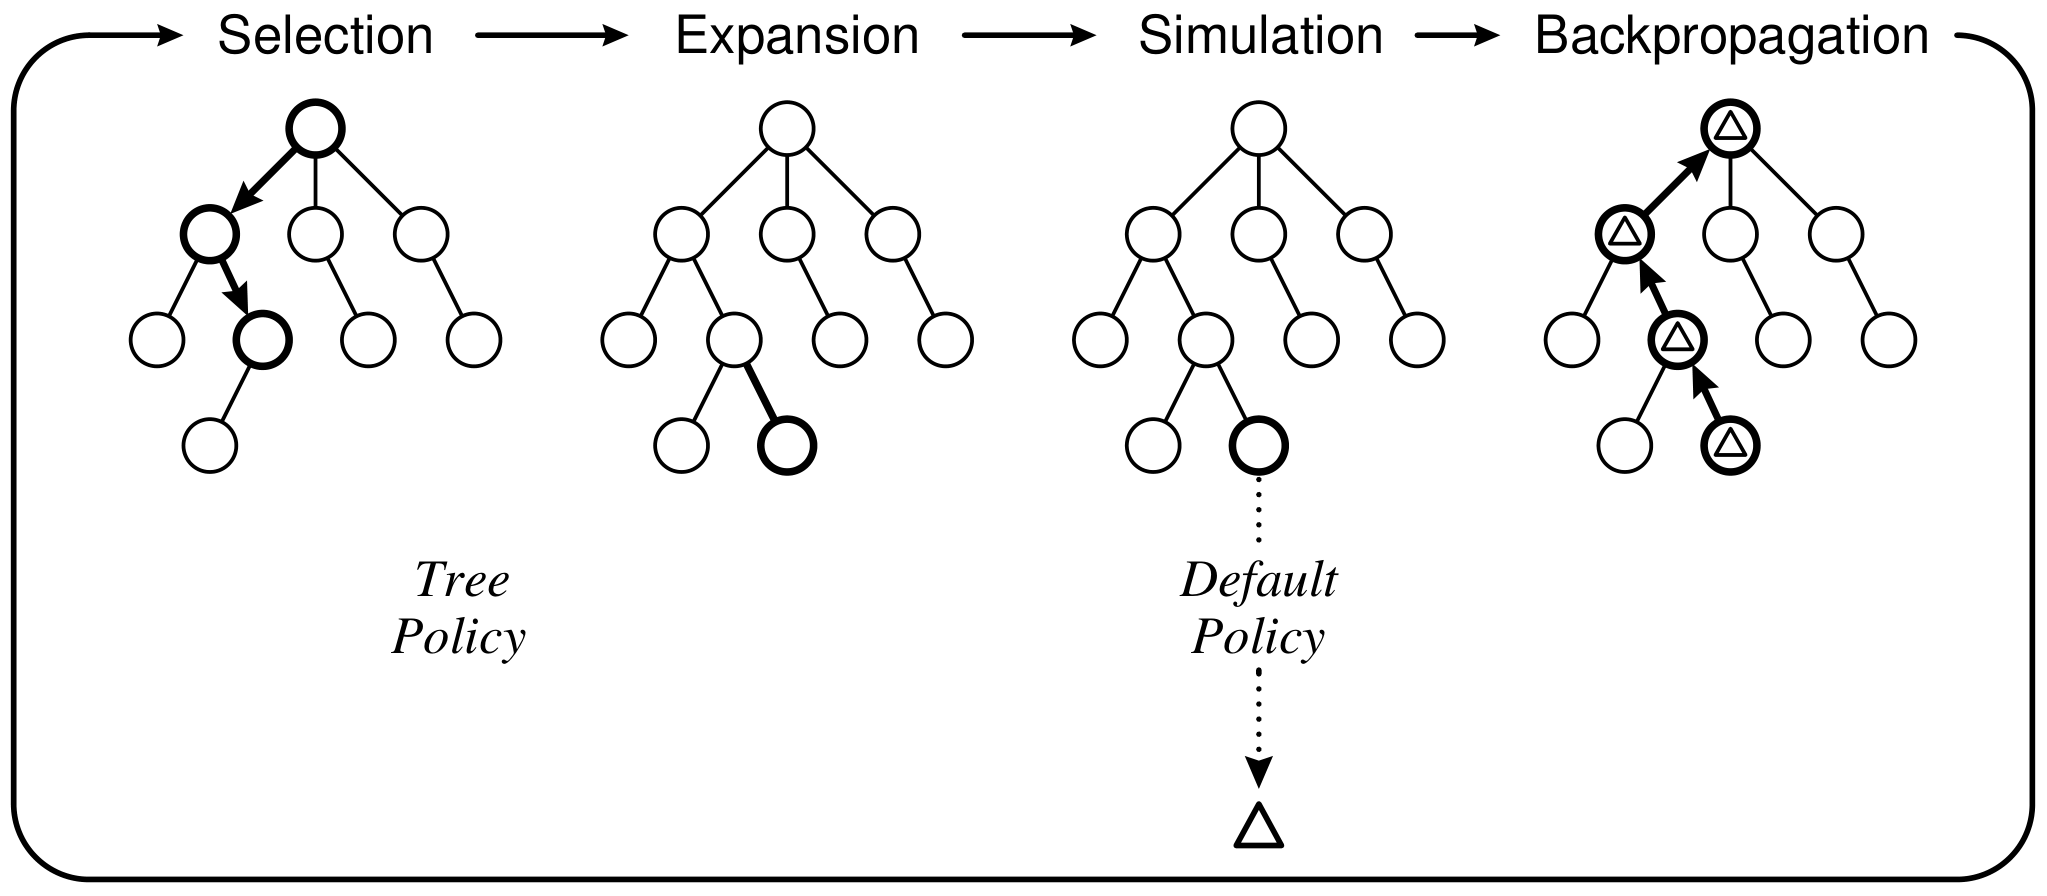
\includegraphics[width=\textwidth]{mcts}
\end{frame}

\begin{frame}{Selection policy}
	\begin{itemize}
		\pause\item Selection must balance:
			\begin{itemize}
				\pause\item \textbf{Exploitation} of moves that are known to be good
				\pause\item \textbf{Exploration} of moves that have not often been tried
			\end{itemize}
		\pause\item This can be modelled as a \textbf{multi-armed bandit problem}
	\end{itemize}
\end{frame}

\begin{frame}{Multi-armed bandits}
	\begin{itemize}
		\pause\item We have a row of one-armed bandits (slot machines)
		\pause\item We \textbf{do not know} the payout probabilities of any of them, and they're all different
		\pause\item How to maximise our winnings?
		\pause\item Again must balance
			\begin{itemize}
				\pause\item \textbf{Exploitation} of machines that are known to have a high expected payout
				\pause\item \textbf{Exploration} of machines that have not been tried often, to get a better estimate of their expected payout
			\end{itemize}
	\end{itemize}
\end{frame}

\begin{frame}{Upper Confidence Bound (UCB)}
	\begin{itemize}
		\pause\item For each machine $m$, record:
			\begin{itemize}
				\pause\item $n_m$: the number of plays of this machine
				\pause\item $V_m$: the total winnings from playing this machine
				\pause\item $n = \sum_m n_m$, total number of plays across all machines
			\end{itemize}
		\pause\item At each stage, play the machine for which
			$$ \frac{V_m}{n_m} + c \sqrt{ \frac{\log n}{n_m} } $$
			is largest
			\begin{itemize}
				\pause\item $\frac{V_m}{n_m}$ is the \textbf{exploitation} part: average payout from this machine so far
				\pause\item $\sqrt{ \frac{\log n}{n_m} }$ is the \textbf{exploration} part: large if $n_m$ is small
				\pause\item $c$ is a parameter for adjusting the balance between exploitation and exploration
			\end{itemize}
	\end{itemize}
\end{frame}

\begin{frame}{UCB demo}
	\begin{center}
		\url{http://orangehelicopter.com/academic/bandits.html?ucb}
	\end{center}
\end{frame}

\begin{frame}{Upper Confidence Bound for Trees (UCT)}
	\begin{itemize}
		\pause\item Use UCB as the selection policy
		\pause\item In each node $x$, record:
			\begin{itemize}
				\pause\item $n_x$: the number of visits to this node
				\pause\item $V_x$: the total value of rollouts through this node
			\end{itemize}
		\pause\item From node $p$, choose the child $q$ such that
			$$ \frac{V_q}{n_q} + c \sqrt{ \frac{\log n_p}{n_q} } $$
			is largest
	\end{itemize}
\end{frame}

\begin{frame}{UCT demo}
\end{frame}

\begin{frame}{Benefits of MCTS}
	\begin{itemize}
		\pause\item ``Vanilla'' MCTS is \textbf{game independent}
		\pause\item But if game-specific heuristics are available, they can be used to \textbf{enhance} MCTS
		\pause\item MCTS is \textbf{anytime}
			\begin{itemize}
				\pause\item Can stop it after \textbf{any} amount of computation (within reason) and get a reasonably good answer
				\pause\item Compare with minimax: $O(e^d)$ for depth $d$
			\end{itemize}
		\pause\item Does not suffer from \textbf{horizon effect}
			\begin{itemize}
				\pause\item Minimax at depth $d$ cannot ``see'' what happens $d+1$ moves in the future
				\pause\item MCTS can build the tree as deep as it likes
				\pause\item Selects which parts of the tree to expand more deeply
			\end{itemize}
	\end{itemize}
\end{frame}

\begin{frame}{MCTS for games of imperfect information}
\end{frame}

